\documentclass[11pt, a4paper]{article}
\usepackage{graphicx}
\usepackage{amsmath}
\usepackage{listings}
\usepackage{minted}

\title{EE6132 Advanced Topics in Signal Processing - Assignment No 2}
\author{
  \textbf{Name}: Atishay Ganesh\\
  \textbf{Roll Number}: EE17B155
}\date{\today}
\begin{document}
		
\maketitle 
\section{Abstract}
The goal of this assignment is the following.
\begin{itemize}
\item To experiment with Convolutional Neural Networks.
\item To study the effects of Batch Normalisation.
\item To visualise the filters and activations of the CNN.
\item To explore adversarial attacks on CNN's.
\end{itemize}
\usemintedstyle{manni}

\section{Assignment}
\subsection{Part 0}
{\bf{Implementation Details:}}{
We use Pytorch in Python 3.6 for implementing the Convolutional Neural Networks. We use torch as the Deep Learning Framework, Tensorboard and pyplot for plotting the graphs and torchvision for the MNIST dataset and the appropriate transforms.
\\\\}

Importing the standard libraries
\begin{minted}[mathescape,escapeinside = ||]{python3}
import sys
import torch
import torch.nn as nn
from torchvision import datasets, transforms
import torch.nn.functional as F
import matplotlib.pyplot as plt
from torch.utils.tensorboard import SummaryWriter
from torch.utils.data import RandomSampler
import numpy as np
from torch.utils.data.sampler import SubsetRandomSampler
from functools import partial
\end{minted}

We write code to load the MNIST Data and split it into train, validation and test sets.(90-10 split)
We normalise the images to -1 to 1.
\begin{minted}[mathescape,escapeinside=||]{python3}
    train_loader = torch.utils.data.DataLoader(
        datasets.MNIST('../data', train=True, download=True,
                       transform=transforms.Compose([
                           transforms.ToTensor(),
                           transforms.Normalize((0.5,), (0.5,))
                       ])),batch_size= batch_size, 
                       shuffle=False,sampler=train_sampler,**kwargs)


\end{minted}

\subsection{MNIST Classifiaction using CNN}
First we construct the CNN Class that will be used for the rest of the assignment.
\\
Forward Pass function:
\begin{minted}{python3}
class CNN(nn.Module):
    def __init__(self,batchnorm=False):
        super(CNN, self).__init__()
        self.batchnorm = batchnorm
        if self.batchnorm:
            self.conv2_bn = nn.BatchNorm2d(32)
            self.fc1_bn = nn.BatchNorm1d(500)
        self.conv1 = nn.Conv2d(in_channels=1,out_channels =32,
        kernel_size= 3, stride = 1,padding=1)
        self.conv2 = nn.Conv2d(in_channels=32, out_channels=32,
        kernel_size= 3, stride = 1,padding=1)
        self.fc1 = nn.Linear(4*4*98, 500)
        self.fc2 = nn.Linear(500, 10)

    def forward(self, x):
        x = F.relu(self.conv1(x))
        x = F.max_pool2d(x, 2, 2)
        x = self.conv2(x)
        if self.batchnorm:
            x = self.conv2_bn(x)
        x = F.relu(x)
        x = F.max_pool2d(x, 2, 2)
        x = x.view(-1, 4*4*98)
        x = (self.fc1(x))

        if self.batchnorm:
            x = self.fc1_bn(x)
        x = F.relu(x)
        x = self.fc2(x)
        return F.log_softmax(x, dim=1)

\end{minted}
\\
We train the network using negative log likelihood loss with optimizer SGD.
\begin{minted}{python3}
    def train_epoch(self,epoch):
        for batch_idx, (data, target) in enumerate(self.train_loader):
            data, target = data.to(self.device), target.to(self.device)
            self.optimizer.zero_grad()
            output = self.model(data)
            correct = 0

            loss = F.nll_loss(output, target)
            pred = output.argmax(dim=1, keepdim=True) 
            correct += pred.eq(target.view_as(pred)).sum().item()

            loss.backward()
            self.optimizer.step()
            self.writer.add_scalar('Loss/train', loss.item(),self.steps)
            self.writer.add_scalar('Accuracy/train',
            100*correct / len(target),self.steps)
            self.steps +=1

            if batch_idx % self.logging_interval == 0:
                print(
                'Train Epoch: {} [{}/{} ({:.0f})%]\tLoss: {:.6f}\n'.format(
                    epoch+1, batch_idx * len(data), self.size[0],
                    100.*batch_idx*len(data) /self.size[0],
                    loss.item()),self.steps)
                self.test_epoch('valid')
                self.model.train()

def test_epoch(self,type_set):
    self.model.eval()
    curr_loader = self.valid_loader if type_set == 'valid' else self.test_loader
    size_value = 1 if type_set =='valid' else 2
    correct = 0
    loss = 0
    with torch.no_grad():
        for data, target in curr_loader:
            data, target = data.to(self.device), target.to(self.device)
            output = self.model(data)
            loss += F.nll_loss(output, target, reduction='sum').item()
            pred = output.argmax(dim=1, keepdim=True) 
            correct += pred.eq(target.view_as(pred)).sum().item()
    loss /= self.size[size_value]
    if type_set== 'valid':

        self.writer.add_scalar('Loss/valid',
                 loss,self.steps)
        self.writer.add_scalar('Accuracy/valid',
                  100.*correct / self.size[size_value],self.steps)

    print('{} set: Average loss: {:.4f}, Accuracy: {}/{} ({:.0f}%)\n'.format(
        type_set,loss, correct, self.size[size_value],
        100.*correct/self.size[size_value]),self.steps)


\end{minted}
\\\\
\subsubsection{Without Batch Normalisation}
We train it with ReLU Non-linearity for 10 epochs.
The results of the same are shown.
\\

Test Set: Average loss: 0.0461, Accuracy: 9845/10000 (98\%)
\\

\begin{figure}[!tbh]
   	\centering
   	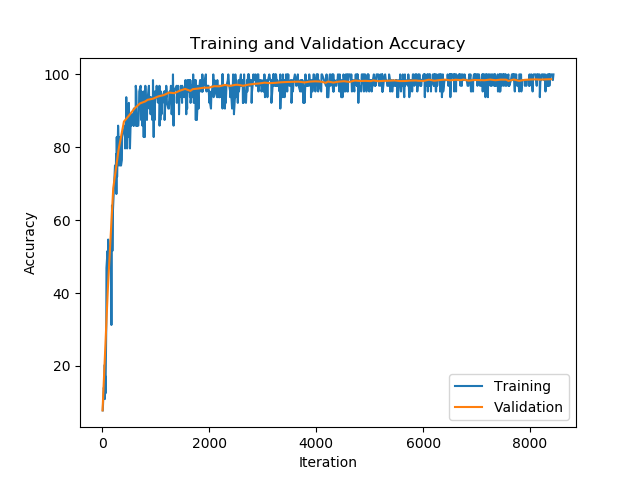
\includegraphics[scale=0.5]{1.png}
   	\caption{Training and Validation Accuracy}
   	\label{fig:1}
   \end{figure}
\begin{figure}[!tbh]
   	\centering
   	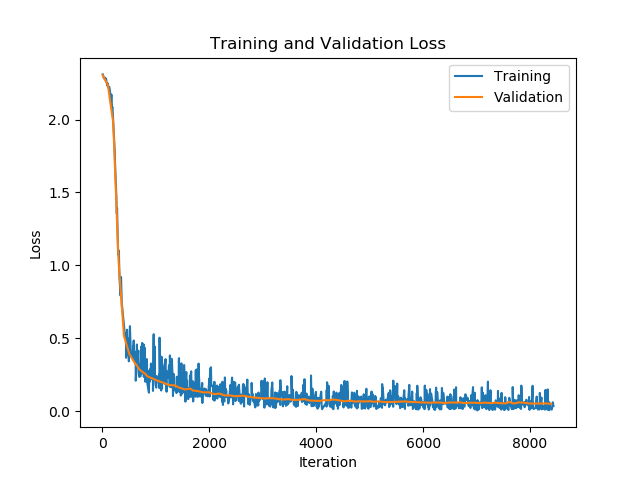
\includegraphics[scale=0.5]{3.png}
   	\caption{Training and Validation Loss}

   	\label{fig:2}
   \end{figure}


\begin{figure}[!th]
\begin{tabular}{lllll}

\includegraphics[scale=2]{Part_12_0.png}
&

\includegraphics[scale=2]{Part_12_1.png}
&

\includegraphics[scale=2]{Part_12_2.png}
&

\includegraphics[scale=2]{Part_12_3.png}
&

\includegraphics[scale=2]{Part_12_4.png}

\end{tabular}
\caption{True Labels: [8,9,5,7,0] Predicted Labels:[8,9,5,7,0] respectively}
\label{Fig:12}
\end{figure}
\\\\

\subsubsection{Description of the CNN}
We list the dimensions of the input and output at each layer. 
\begin{itemize}
    \item Conv1 Input: 1,28,28 Output: 32,28,28
    \item Maxpool Input: 32,28,28 Output: 32,14,14
    \item Conv2 Input: 32,14,14 Output: 32,14,14
    \item Maxpool Input: 32,14,14 Output: 32,7,7
    \item Linear 1 Input: 1568 Output: 500
    \item Linear 2 Input: 500 Output: 10
\end{itemize}
We discuss the number of parameters in our network
\begin{itemize}
    \item Conv1: 320 (288 Weights + 32 Biases)
    \item Conv2: 9248 (9216 Weights +32 Biases)
    \item Linear1: 784500 (784000 Weights and 500 Biases)
    \item Linear2: 5010 (5000 Weights and 10 Biases)
\end{itemize}
9568 Parameters belong to the convolutional layers.
789510 Parameters belong to the fully connected layers.
\\
The number of neurons in our network is
\begin{itemize}
    \item Conv1: 25088 Neurons
    \item Conv2: 25088 Neurons
    \item Linear1: 500 Neurons
    \item Linear2: 10 Neurons
\end{itemize}
50176 Neurons belong to the convolutional layers.
510 Neurons belong to the fully connected layers.
\\

\subsubsection{Batch Normalization}
We use batch normalization between conv2 and its relu, and Linear 1 and its relu.
The use of batch normalization was initially introduced to combat the effect of the internal covariate shift. However, recent studies state that batch normalization smoothens the optimization landscape, and this is reason the performance is better.
Test Set: Average loss: 0.0316, Accuracy: 9897/10000 (99\%)
Batch-normalization improved the test accuracy by a small amount that was reducing as the network trained more, and the training time to reach a certain validation accuracy threshold did reduce by a good amount.
The conditions were same as the previous case.
\\
\begin{figure}[!tbh]
   	\centering
   	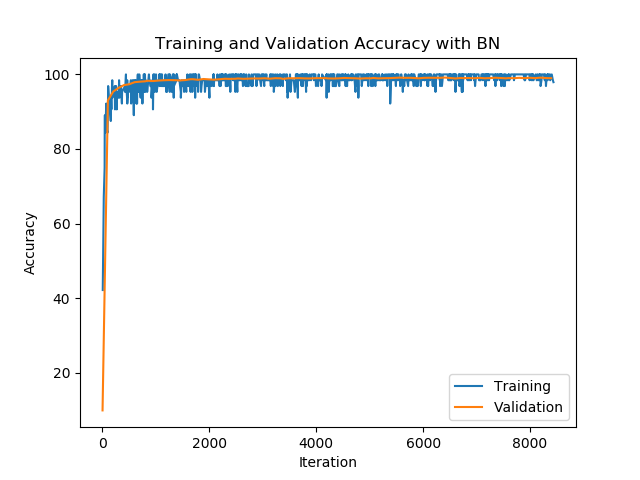
\includegraphics[scale=0.5]{5.png}
   	\caption{Training and Validation Accuracy}
   	\label{fig:3}
   \end{figure}
\begin{figure}[!tbh]
   	\centering
   	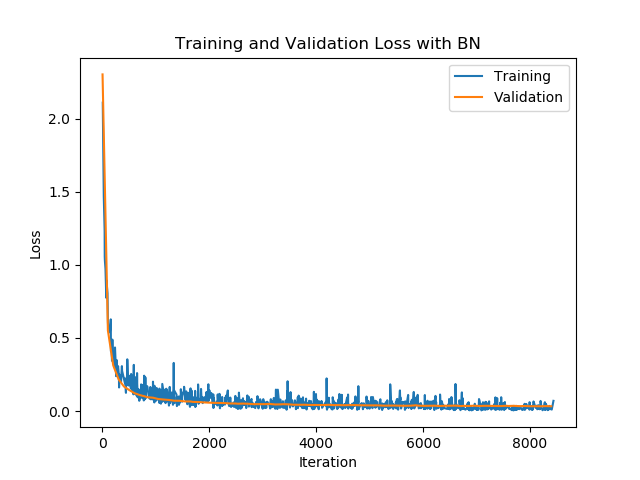
\includegraphics[scale=0.5]{7.png}
   	\caption{Training and Validation Loss}

   	\label{fig:4}
   \end{figure}
\begin{figure}[!tbh]
   	\centering
   	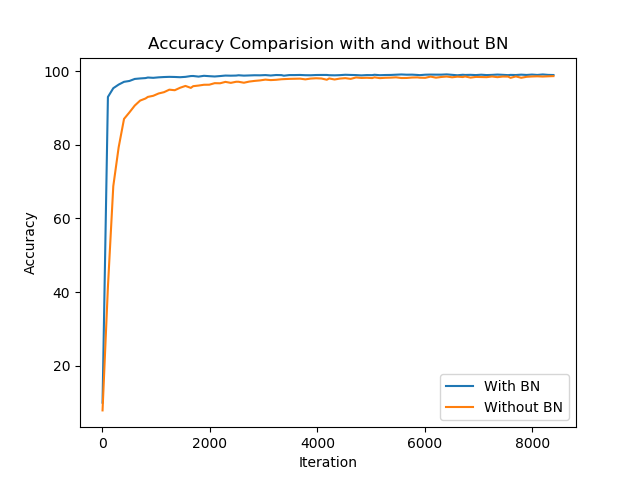
\includegraphics[scale=0.5]{9.png}
   	\caption{Accuracy with and without Batch Norm}
   	\label{fig:5}
   \end{figure}
\begin{figure}[!tbh]
   	\centering
   	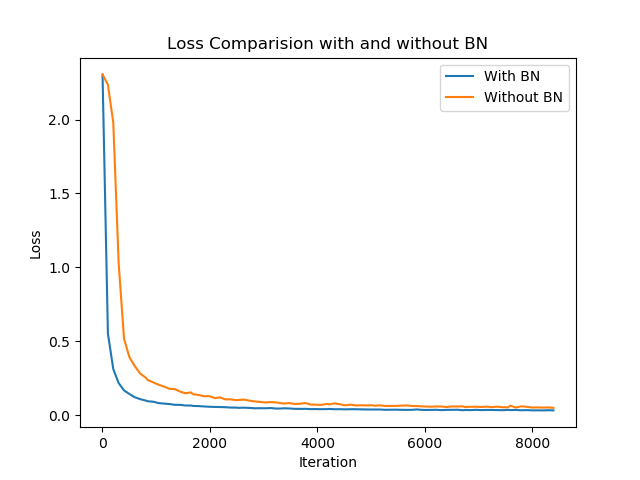
\includegraphics[scale=0.5]{11.png}
   	\caption{ Loss with and without Batch Norm}

   	\label{fig:6}
   \end{figure}



\subsection{Visualing Convolutional Neural Networks}
\subsubsection{Plot filters}
{We observe certain patterns which are difficult to interpret as such, since the filter size is extremely small. If the filter size was higher we would expect the first layer to have patterns like a sobel filter. The later layers do not much visual significance.}
\\
\begin{figure}[!th]
\begin{tabular}{lllll}
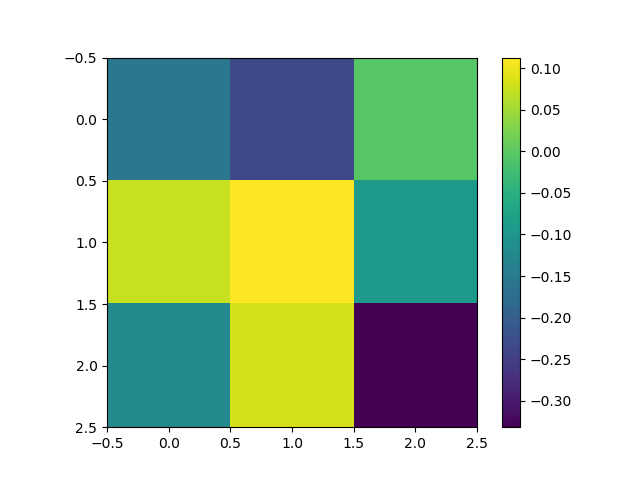
\includegraphics[scale=0.125]{Part_20_0_conv1.png}
&
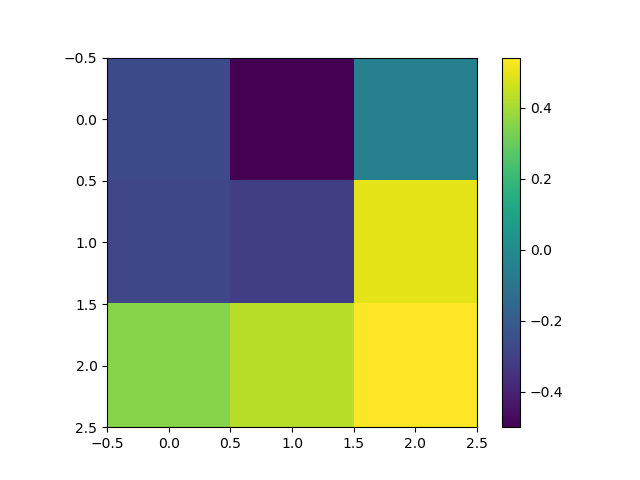
\includegraphics[scale=0.125]{Part_20_1_conv1.png}
&
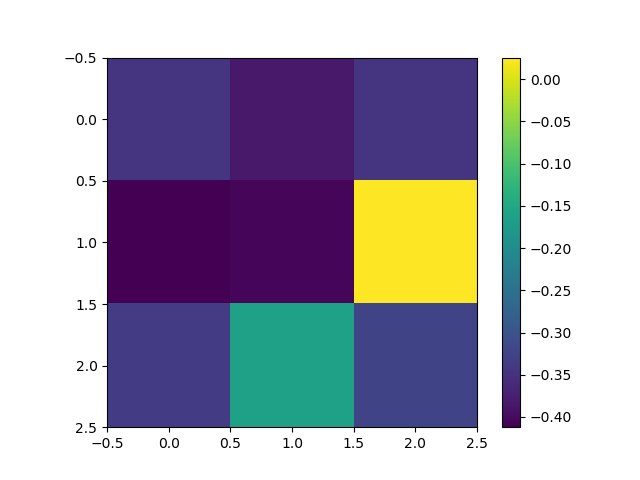
\includegraphics[scale=0.125]{Part_20_2_conv1.png}
&
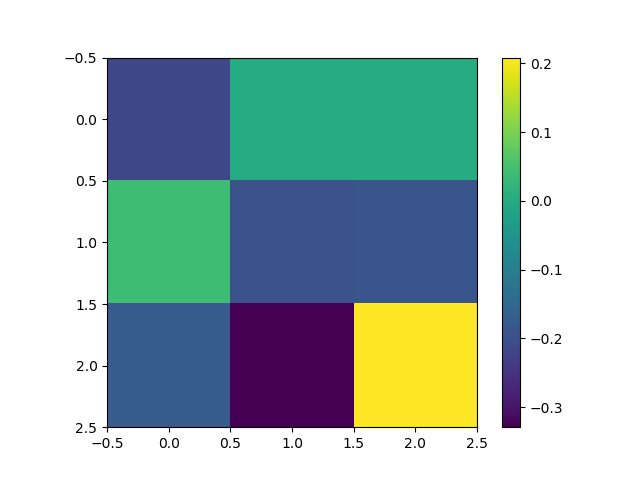
\includegraphics[scale=0.125]{Part_20_3_conv1.png}
&
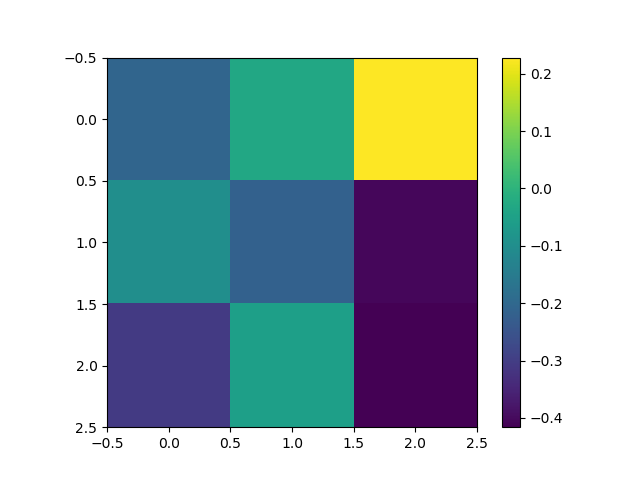
\includegraphics[scale=0.125]{Part_20_4_conv1.png}

\end{tabular}
\caption{Filters from First Convolutional Layer}
\label{Fig:20}
\end{figure}

\begin{figure}[!th]
\begin{tabular}{lllll}
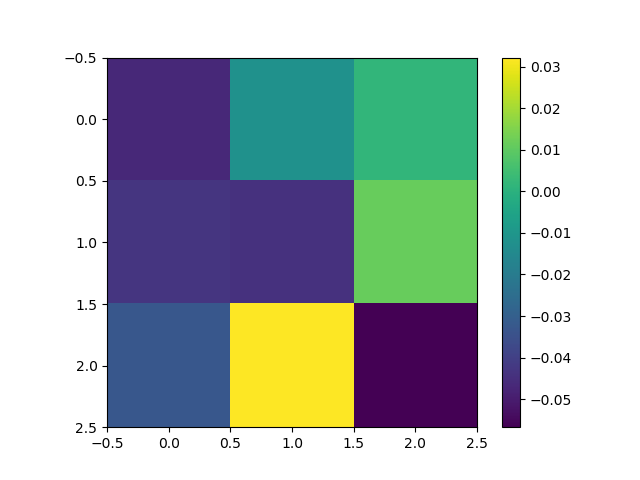
\includegraphics[scale=0.125]{Part_20_0_conv2.png}
&
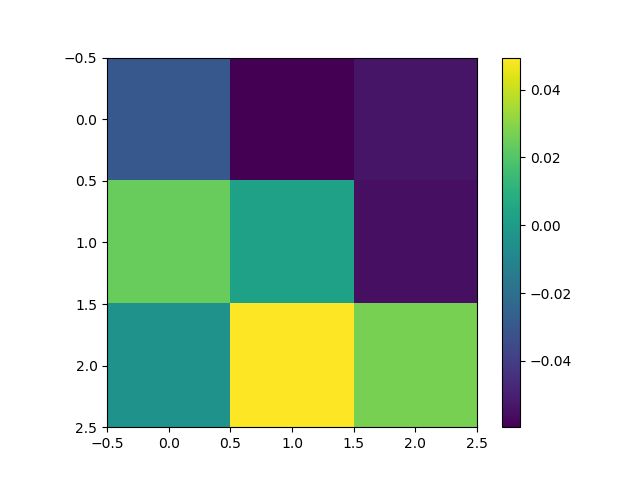
\includegraphics[scale=0.125]{Part_20_1_conv2.png}
&
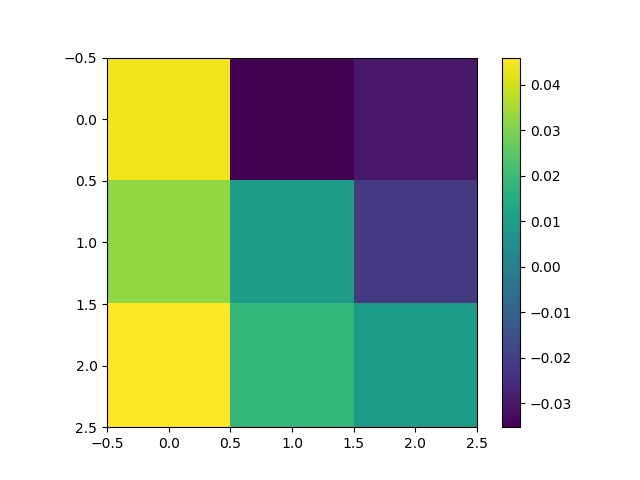
\includegraphics[scale=0.125]{Part_20_2_conv2.png}
&
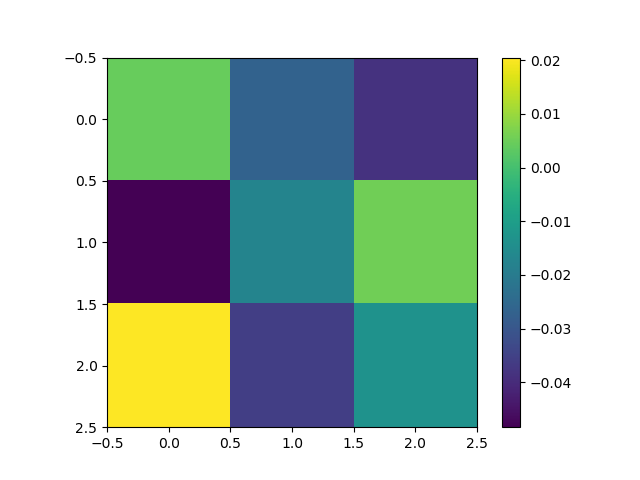
\includegraphics[scale=0.125]{Part_20_3_conv2.png}
&
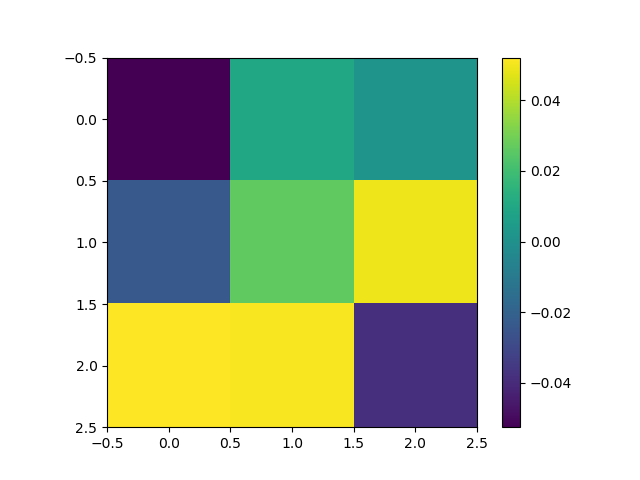
\includegraphics[scale=0.125]{Part_20_4_conv2.png}

\end{tabular}
\caption{Filters from Second Convolutional Layer}
\label{Fig:21}
\end{figure}


\\\\


\subsubsection{Visualising Activations}
We Visualise some of the activations of the convolutional layers. As we go deeper the activations get smaller and the activations itself are not so clear, but the digit can still be made out in the second layer.
\\


\begin{figure}[!th]
\begin{tabular}{lllll}

\includegraphics[scale=2]{Part_21_0_conv1.png}
&

\includegraphics[scale=2]{Part_21_1_conv1.png}
&

\includegraphics[scale=2]{Part_21_2_conv1.png}
&

\includegraphics[scale=2]{Part_21_3_conv1.png}
&

\includegraphics[scale=2]{Part_21_4_conv1.png}

\end{tabular}
\caption{Activations from First Convolutional Layer}
\label{Fig:20}
\end{figure}

\begin{figure}[!th]
\begin{tabular}{lllll}

\includegraphics[scale=2]{Part_21_0_conv2.png}
&

\includegraphics[scale=2]{Part_21_1_conv2.png}
&

\includegraphics[scale=2]{Part_21_2_conv2.png}
&

\includegraphics[scale=2]{Part_21_3_conv2.png}
&
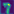
\includegraphics[scale=2]{Part_21_4_conv2.png}

\end{tabular}
\caption{Activations from Second Convolutional Layer}
\label{Fig:21}
\end{figure}




\subsubsection{Occlusion of Image}
In this part we occlude parts of the image to test if the learning is proper.
With a gray patch of 5x5, we observe that in most cases the probability is pretty good, but when it over the image, the probabilities of the class reduce, in one particular case it reduced dramatically, presumably since the digit in question there (7) looked quite similar to 1. Hence it appears the neural network is learning quite well.
It is interesting to observe that when we occlude at the digit or near the digit, the probability of the class decreases quite a lot. The probability of the class does not decrease too much as the patch is relatively small,but with a larger patch size it would decrease more substansially. 
\\
\begin{figure}[!th]
\begin{tabular}{ll}
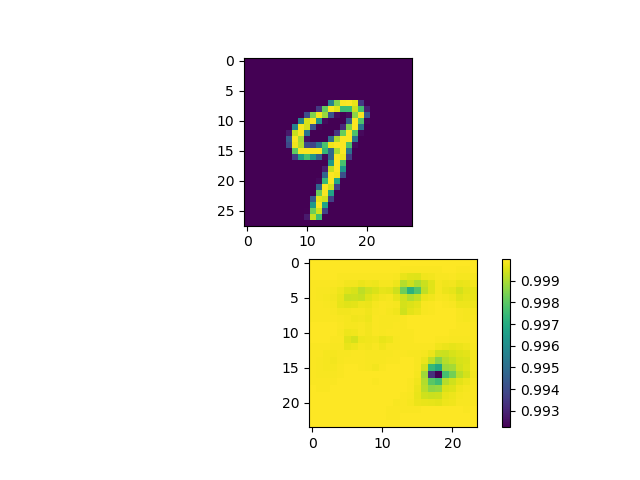
\includegraphics[scale=0.3]{Part_22_0.png}
&
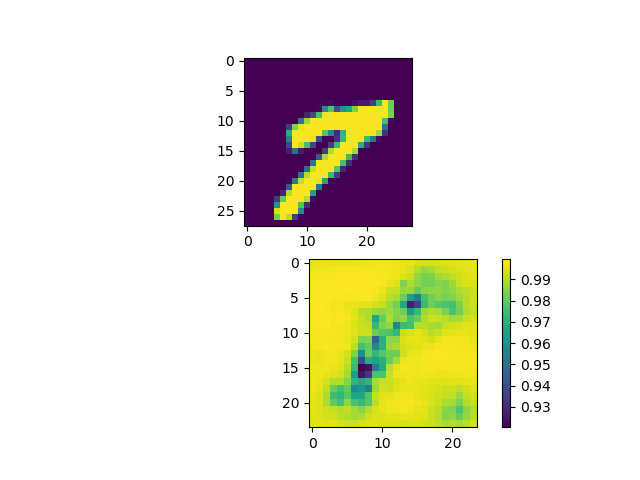
\includegraphics[scale=0.3]{Part_22_1.png}
&
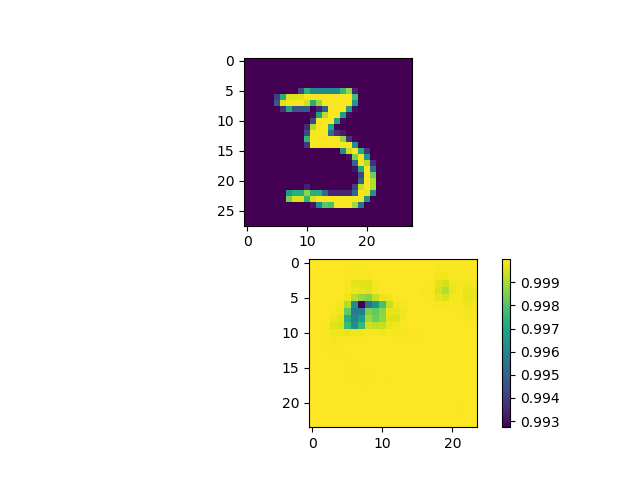
\includegraphics[scale=0.3]{Part_22_2.png}
&
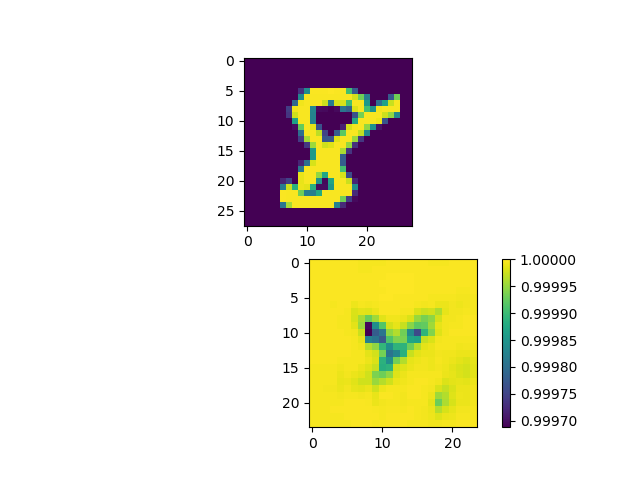
\includegraphics[scale=0.3]{Part_22_3.png}
&
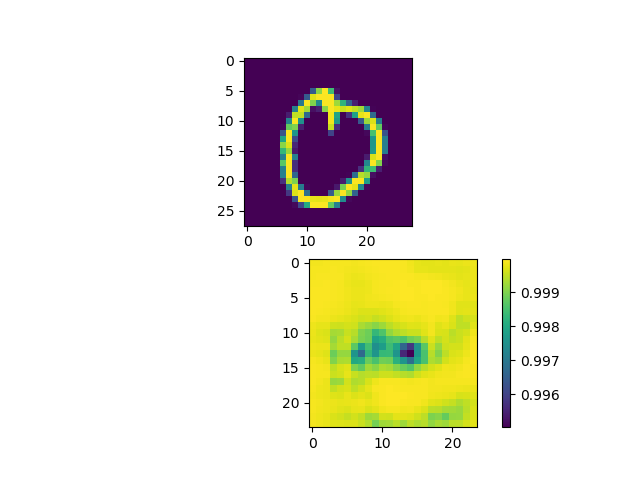
\includegraphics[scale=0.3]{Part_22_4.png}
&
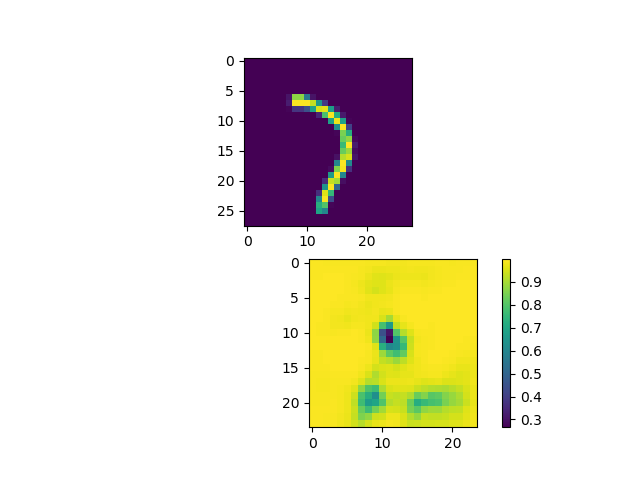
\includegraphics[scale=0.3]{Part_22_5.png}
&
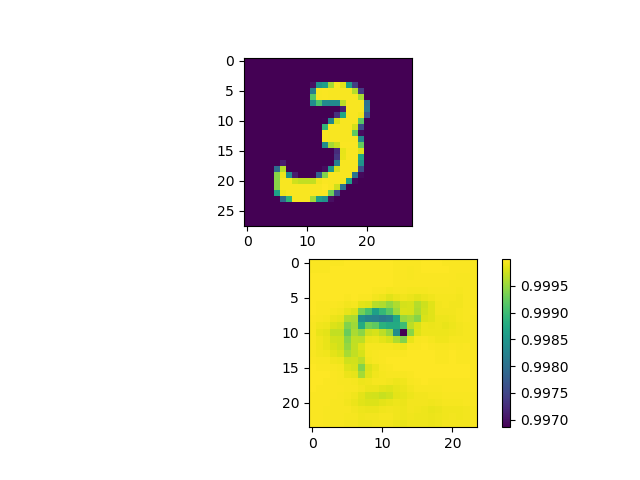
\includegraphics[scale=0.3]{Part_22_6.png}
&
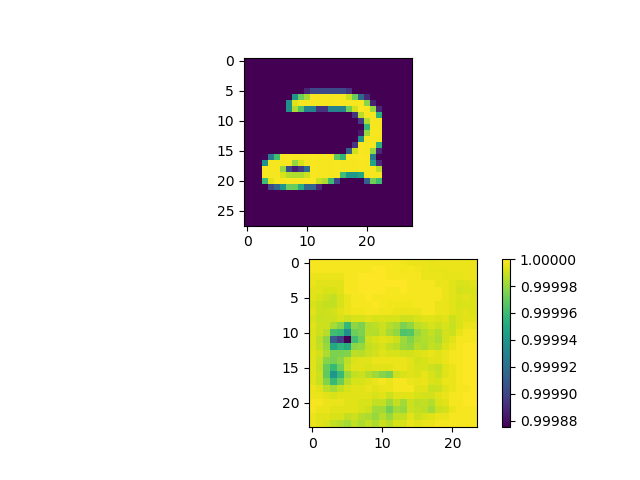
\includegraphics[scale=0.3]{Part_22_7.png}
&
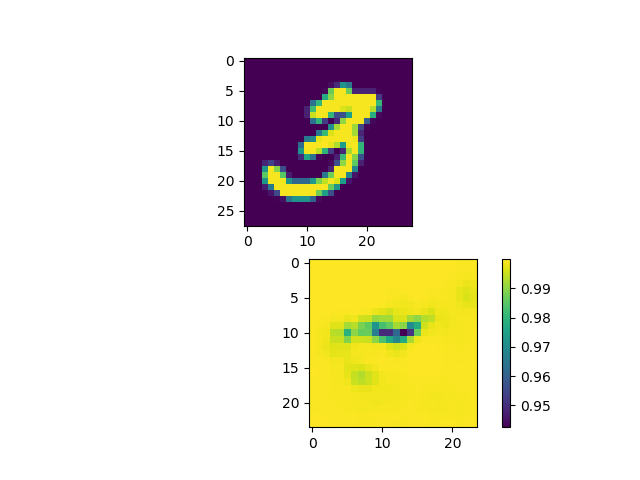
\includegraphics[scale=0.3]{Part_22_8.png}
&
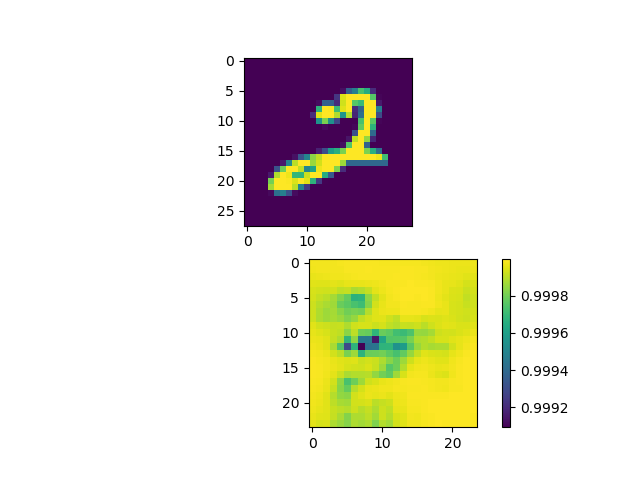
\includegraphics[scale=0.3]{Part_22_9.png}

\end{tabular}
\caption{Probabilities after occluding parts of the image.}
\label{Fig:25}
\end{figure}


\subsection{Adversarial Examples}
We load one of the MNIST models from the first question and try and construct adversarial examples for the network.
\subsubsection{Non Targeted Attack}
We try to make a matrix with noise that will be classified by the network as some class with 99\% probability. 
The plotting code is emitted from the code snippet for brevity reasons.
\begin{minted}{python3}
    elif sys.argv[1] == 'Part_30':
        '''Non Targeted Attack'''
        X = np.random.normal(0,0.1,(1,1,28,28))
        X = X.astype('d')
        X = np.clip(X,-1,1)
        model = CNN()
        model.load_state_dict(torch.load('mnist_cnn.pt'))
        model.train()
        step = 0.1
        for i in range(10):
            p = 0
            print(X.shape)
            z = np.array([i])
            target =torch.from_numpy(z).type('torch.LongTensor')

            X1 = torch.tensor(X, requires_grad=True).type('torch.FloatTensor')
            device = torch.device( "cpu")
            plist= []
            while(p<0.99):
                X1, target = X1.to(device), target.to(device)
                loss = model.forward_logits(X1)
                prob = model(X1)
                p = np.exp(prob.detach().numpy())[0,i]
                g = torch.autograd.grad(loss[0][i],X1)
                X1 = X1+step*g[0]
                print(p)
                plist.append(loss[0][i].detach().numpy())
\end{minted}
\begin{figure}[!th]
\begin{tabular}{lllll}
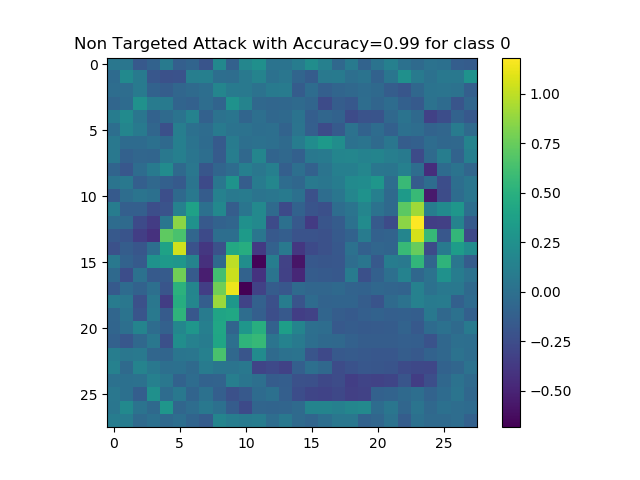
\includegraphics[scale=0.125]{Part_30_0_99.png}
&
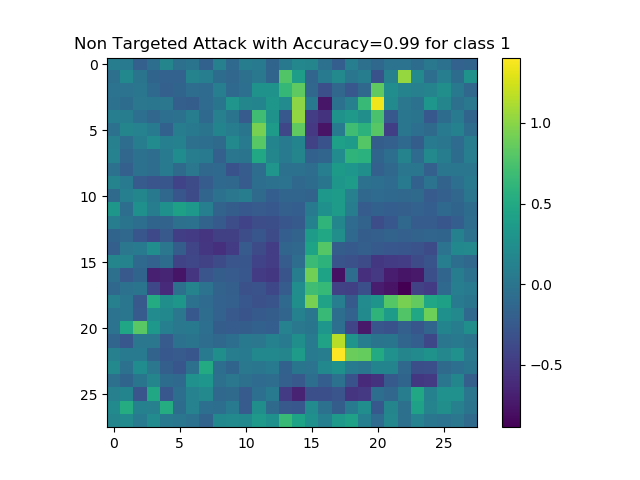
\includegraphics[scale=0.125]{Part_30_1_99.png}
&
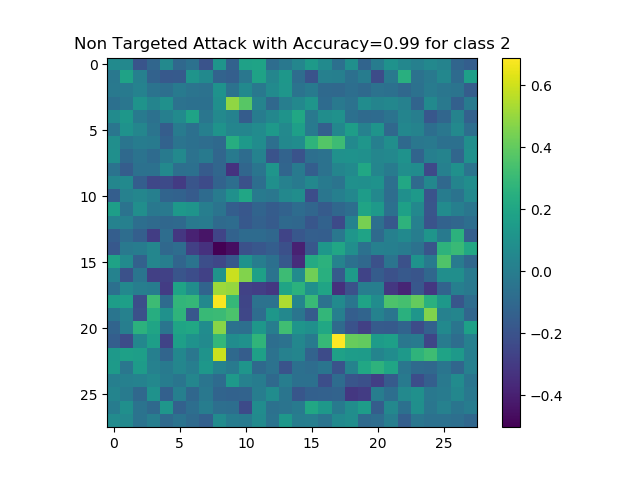
\includegraphics[scale=0.125]{Part_30_2_99.png}
&
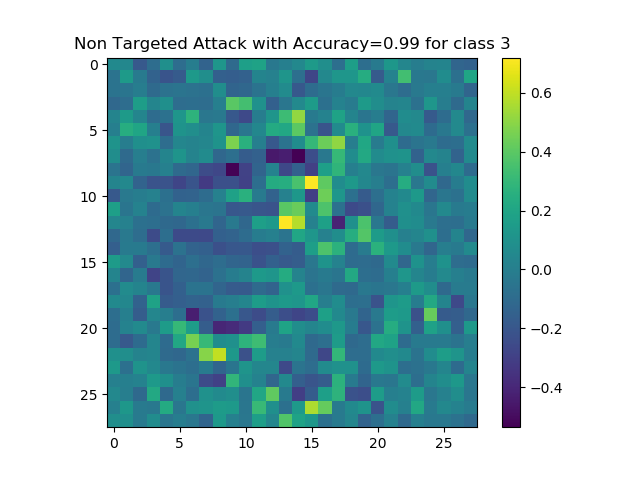
\includegraphics[scale=0.125]{Part_30_3_99.png}
&
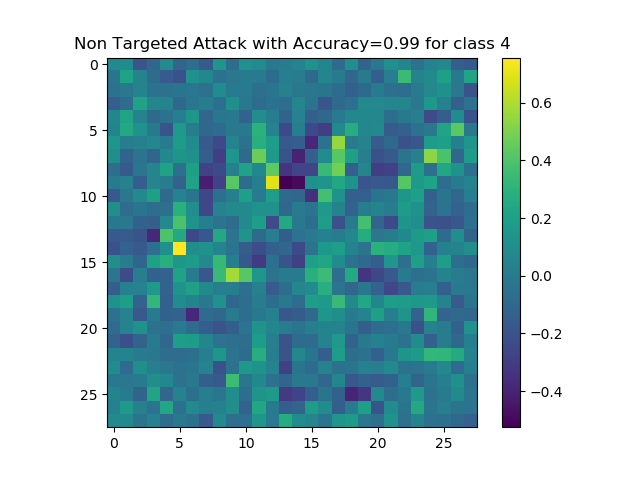
\includegraphics[scale=0.125]{Part_30_4_99.png}
&
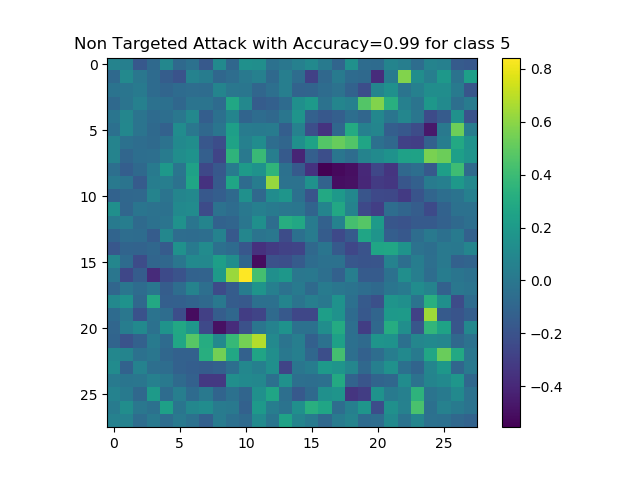
\includegraphics[scale=0.125]{Part_30_5_99.png}
&
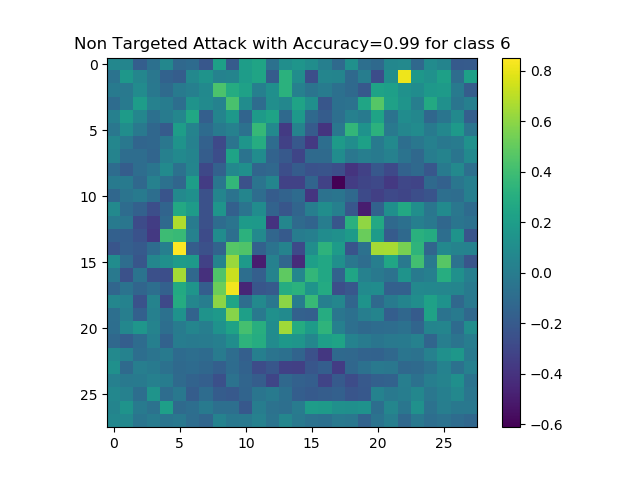
\includegraphics[scale=0.125]{Part_30_6_99.png}
&
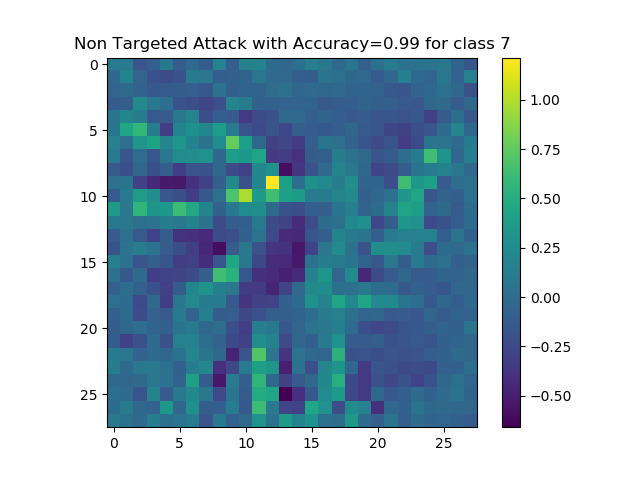
\includegraphics[scale=0.125]{Part_30_7_99.png}
&
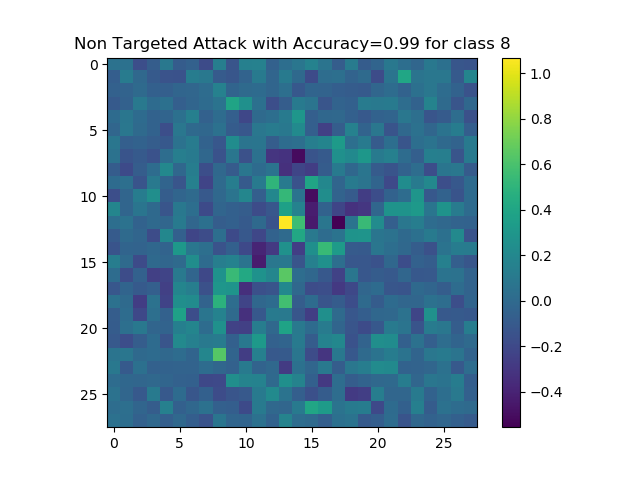
\includegraphics[scale=0.125]{Part_30_8_99.png}
&
\includegraphics[scale=0.125]{Part_30_9_99.png}

\end{tabular}
\caption{Non Targeted Attacks for 0-9 target classes (Row Major).}
\label{Fig:30}
\end{figure}
\begin{itemize}
    \item Yes, because we have trained it till it predicts target\_class with high confidence.
    \item No. They do not look like a number but mostly noise. The network has not been trained on these mostly noise images, hence it predicts without too much logic, hence we can pass off random noise as numbers. 
    \item We observe that the cost is linearly increasing.
\end{itemize}

\begin{figure}[!tbh]
   	\centering
   	\includegraphics[scale=0.5]{Part_30_1_cost.png}
   	\label{fig:31}
   \caption{Class 1 output cost}
   \end{figure}
\subsubsection{Analysis}

\begin{figure}[!tbh]
   	\centering
   	\includegraphics[scale=0.5]{Part_30_7_cost.png}
   	\label{fig:32}
   \caption{Class 7 output cost}
   \end{figure}

\subsubsection{Targeted Attack}
We generate some adversarial example that looks like a particular
digit, which the network classifies as another digit with 90\% probability.
\\
Relavant Code Snippet
\begin{minted}{python3}
    
    while(p<0.90):
        X1 = X1.to(device)
        loss = model.forward_logits(X1)[0][target] - beta*F.mse_loss(
                start_image,target_image)
        prob = model(X1)
        p = np.exp(prob.detach().numpy())[0,target]
        g = torch.autograd.grad(loss,X1)
        X1 = X1+step*g[0]
        print(p)

\end{minted}
The images now look like the original image but are classified as the target image.
All images have been created and are in the submission, but for brevity only 1 per input class and 1 per target class are included in this report.


\begin{figure}[!th]
\begin{tabular}{lllll}
\includegraphics[scale=0.125]{Part_31_0to5_99.png}
&
\includegraphics[scale=0.125]{Part_31_1to4_99.png}
&
\includegraphics[scale=0.125]{Part_31_2to3_99.png}
&
\includegraphics[scale=0.125]{Part_31_3to2_99.png}
&
\includegraphics[scale=0.125]{Part_31_4to6_99.png}
&
\includegraphics[scale=0.125]{Part_31_5to1_99.png}
&
\includegraphics[scale=0.125]{Part_31_6to7_99.png}
&
\includegraphics[scale=0.125]{Part_31_7to9_99.png}
&
\includegraphics[scale=0.125]{Part_31_8to0_99.png}
&
\includegraphics[scale=0.125]{Part_31_9to8_99.png}

\end{tabular}
\caption{Targeted Attack: True Label:[0,1,2,3,4,5,6,7,8,9] \\        Predicted Label:[5,4,3,2,6,1,7,9,0,8]}
\label{Fig:33}
\end{figure}
The Generated Images look similar to the original images but with some amount of noise or blur.

\subsubsection{Adding noise}
We try to add noise to fool the network.

Relevant Code Snippet:
\begin{minted}{python3}
    while(p<0.99):
        X2 = X2.to(device)
        loss = model.forward_logits(X2)[0][target]
        prob = model(X2)
        p = np.exp(prob.detach().numpy())[0,target]
        g = torch.autograd.grad(loss,X3)
        X3 = X3+step*g[0]
        X2 = X1 +X3
        print(p)

\end{minted}



\begin{figure}[!th]
\begin{tabular}{lll}
\includegraphics[scale=0.25]{Part_32_0to1_99.png}
&
\includegraphics[scale=0.25]{Part_32_1to2_99.png}
&
\includegraphics[scale=0.25]{Part_32_2to3_99.png}
&
\includegraphics[scale=0.25]{Part_32_4to5_99.png}
&
\includegraphics[scale=0.25]{Part_32_5to6_99.png}
&
\includegraphics[scale=0.25]{Part_32_6to7_99.png}
&
\includegraphics[scale=0.25]{Part_32_7to8_99.png}
&
\includegraphics[scale=0.25]{Part_32_7to8_99.png}
&
\includegraphics[scale=0.25]{Part_32_8to9_99.png}
&
\includegraphics[scale=0.25]{Part_32_9to0_99.png}

\end{tabular}
\caption{Attack with noise. The true labels :[0-9]\\        Predicted Labels: True Label +1 (mod 10)\\      The Top image is the adversarial example and the bottom one is the noise}
\label{Fig:33}
\end{figure}

The noise got from the noise attack can be added to other examples to fool the network, but it does not seem to be very robust.

Noise Targets:\\
$[1, 2, 3, 4, 5, 6, 7, 8, 9, 0]$\\
True Image:\\
$[8, 5, 0, 9, 7, 1, 3, 1, 9, 3]$\\
Predictions\\
(each row is all the true images for a single noise target.)\\
$$
 \begin{bmatrix} 
1 & 3 & 1 & 1 & 2 & 1 & 3 & 1 & 1 & 3 \\
2 & 2 & 0 & 2 & 2 & 2 & 2 & 2 & 8 & 2 \\
8 & 8 & 0 & 9 & 7 & 1 & 3 & 3 & 9 & 3 \\
8 & 5 & 0 & 4 & 7 & 8 & 9 & 4 & 9 & 9 \\
8 & 5 & 0 & 9 & 9 & 5 & 3 & 9 & 9 & 5 \\
8 & 8 & 0 & 4 & 7 & 1 & 3 & 1 & 9 & 3 \\
8 & 5 & 0 & 9 & 7 & 7 & 3 & 3 & 9 & 3 \\
8 & 8 & 0 & 8 & 8 & 8 & 3 & 8 & 8 & 3 \\
8 & 5 & 0 & 9 & 7 & 8 & 3 & 9 & 9 & 3 \\
8 & 8 & 0 & 8 & 7 & 0 & 3 & 0 & 9 & 3 \\
  \end{bmatrix}
 $$
In a good number of cases the network is fooled by adding the noise, to predict the noise target instead of the True output. This method does not appear to be infallible, but it does very well at times, especially for 2,8,1 in that order.
\section{Conclusions}
\begin{itemize}
\item We experimented with Convolutional Neural Networks for image classification.
\item We studied the effects of Batch Normalisation in improving the performance of the neural network.
\item We visualised the filters and activations of the CNN.
\item We explored adversarial attacks on CNN's (targeted, non targeted and noise driven attacks).
\end{itemize}



\bibliography{website} 
\bibliographystyle{ieeetr}
\end{document}



 